%%%%%%%%%%%%%%%%%%%%%%%%%%%%%%%%%%%%%%%%%%%%%%%%%%%%%%%%%%%%%%%%%%%%
%% %%	Posterdown PDF class for LaTeX files	 08-JAN-2019
%% %%	For any information please send an e-mail to:
%% %%		brentthonre18@gmail.com (Brent Thorne)
%% %%
%% %%	Initial class provided by:
%% %%		Brent Thorne
%% %% Contributors: Shea Connell (SC)
%%%%%%%%%%%%%%%%%%%%%%%%%%%%%%%%%%%%%%%%%%%%%%%%%%%%%%%%%%%%%%%%%%%%

\documentclass[article,30pt,extrafontsizes]{memoir}

%utf-8 seems to be important
\RequirePackage[utf8]{inputenc}
\RequirePackage[T1]{fontenc}
\RequirePackage{lmodern}
\RequirePackage{multicol}
\RequirePackage{graphicx}
\RequirePackage{lipsum}
\RequirePackage{blindtext}
\RequirePackage[svgnames,table]{xcolor}
\RequirePackage{tikz}
\RequirePackage[framemethod=tikz]{mdframed}
\RequirePackage{color}
\RequirePackage{geometry}
\RequirePackage{adjmulticol}
\RequirePackage[skins,most,listings,skins]{tcolorbox}

%For kable extra package :)
\RequirePackage{booktabs}
\RequirePackage{longtable}
\RequirePackage{array}
\RequirePackage{multirow}
\RequirePackage{wrapfig}
\RequirePackage{float}
\RequirePackage{colortbl}
\RequirePackage{pdflscape}
\RequirePackage{pagecolor}
\RequirePackage{tabu}
\RequirePackage{threeparttable}
\RequirePackage{threeparttablex}
\RequirePackage[normalem]{ulem}
\RequirePackage{makecell}
\RequirePackage{wrapfig}

%rof hyperrefs
\RequirePackage{hyperref}
\hypersetup{
    colorlinks=true,
    linkcolor=linkcol,
    citecolor=citecol,
    filecolor=linkcol,
    urlcolor=urlcol,
}
%For figure and table placement
\RequirePackage{float}
\floatplacement{figure}{H}
\floatplacement{table}{H}

%%%%%%%%% COLOURS %%%%%%%%
%Fill/ Line Colours
\definecolor{titleboxbgcol}{HTML}{537c8e}
\definecolor{titleboxbordercol}{HTML}{2ebdbd}
\definecolor{columnlinecol}{HTML}{537c8e}
\definecolor{bodybgcol}{HTML}{ffffff}
\definecolor{sectitlebgcol}{HTML}{2ebdbd}
\definecolor{sectitlebordercol}{HTML}{2ebdbd}
% Text Colours
\definecolor{titletextcol}{HTML}{ffffff}
\definecolor{authortextcol}{HTML}{ffffff}
\definecolor{affiliationtextcol}{HTML}{FFFFFF}
\definecolor{sectitletextcol}{HTML}{ffffff}
\definecolor{bodytextcol}{HTML}{000000}
\definecolor{footnotetextcol}{HTML}{ffffff}
\definecolor{citecol}{HTML}{CC0000}
\definecolor{urlcol}{HTML}{537c8e}
\definecolor{linkcol}{HTML}{537c8e}


%Memoir spacing options
%spacing between figure/ table and caption
\setlength{\abovecaptionskip}{0.4in}
\setlength{\belowcaptionskip}{0.2in}
\captionnamefont{\footnotesize\sffamily\bfseries}
\captiontitlefont{\footnotesize\sffamily}

%define column options
\setlength{\columnseprule}{0.5pt}
\def\columnseprulecolor{\color{columnlinecol}}

%define section title features
\setsubsubsecheadstyle{\small\color{sectitletextcol}\textbf}% Set \section style
\setsecnumformat{}
\def\sectionmark#1{\markboth{#1}{#1}}

%%%%%%%%%%%% TCOLORBOXES TO THE RESCUE %%%%%%%%%%%%%%%%%%%%
%Title Box
\newtcolorbox{topbox}{
enhanced,
colback=titleboxbgcol,
colframe=titleboxbordercol,
halign=center,
boxrule=1cm,
sharp corners=all,
 overlay={
    \node[anchor=south west]
      at ([xshift=100in,yshift=0.2in]frame.south west)
       {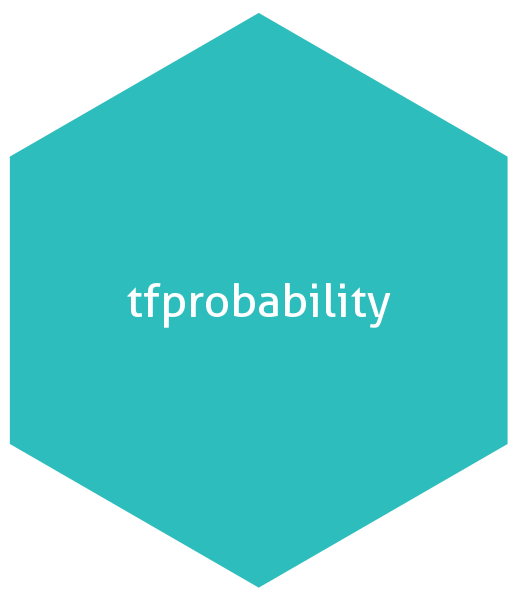
\includegraphics[width=3in]{tfprobability.png}};
    \node[anchor=south east]
      at ([xshift=-0.5in,yshift=0.2in]frame.south east)
       {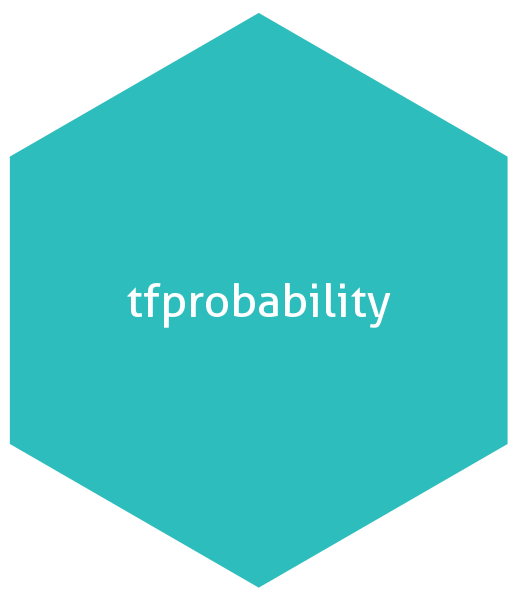
\includegraphics[width=3in]{tfprobability.png}};}

}
%Body Section Title Box
\newtcolorbox{myboxstuff}[1][]{
code={\parindent=0em},
colframe=sectitlebordercol,
nobeforeafter,
left skip=0pt,
valign=center,
halign=center,
fontupper=\Large\bfseries,
colupper=sectitletextcol,
boxrule=2mm,
colback=sectitlebgcol,
sharp corners=uphill, #1}
\newcommand{\mybox}[1]{%
\begin{myboxstuff}
\strut #1
\end{myboxstuff}%
}
\makeheadstyles{MyBox}{
    \setsecheadstyle{\mybox}
}
\headstyles{MyBox}\makepagestyle{MyBox}
%-----------------------------------------------------
%Make sure that the page is empty of any preset items from memoir
\thispagestyle{empty}

%biblatex options
\RequirePackage[sorting=none,backend=biber]{biblatex}
\renewcommand*{\bibfont}{\small} %% SC
\bibliography{MyLibrary}
\defbibheading{bibliography}[\bibname]{%
\setlength\bibitemsep{0.8\itemsep} %% SC
\section*{#1}%
\markboth{#1}{#1}}
\AtBeginDocument{%
  \renewcommand{\bibname}{References}
}

%Remove section numbering & set 2nd level header as first level
%to avoid the automatic new page generated from memoir chapter
%formatting
\counterwithout{section}{chapter}
\makechapterstyle{mydefault}{
\addtocounter{secnumdepth}{2}
\setsecheadstyle{\mybox}
\setsubsecheadstyle{\itshape}
\setsubsubsecheadstyle{\itshape}
}

%set the chapterstyle
\chapterstyle{mydefault}

%define column spacing
\setlength\columnsep{0.5in}

%spacing params
\setlength\parindent{0em}
\setlength\parskip{0em}
\setlength\hangparas{0}

%spacing after section head title
\setaftersecskip{0em}
\setbeforesecskip{1.5em}
\setlength\textfloatsep{0in}
\setlength\floatsep{0in}
\setlength\intextsep{0in}

\setstocksize{46.8in}{33.1in}
\settrimmedsize{\stockheight}{\stockwidth}{*}
\settypeblocksize{46.8in}{33.1in}{*}
\setlrmargins{*}{*}{1}
\setulmarginsandblock{2.5cm}{*}{*}
\setmarginnotes{0em}{0cm}{0cm}
\setlength{\footskip}{0cm}
\setlength{\footnotesep}{0cm}
\setlength{\headheight}{0pt}
\setlength{\headsep}{0pt}
\setlength{\trimtop}{0pt}
\setlength{\trimedge}{0pt}
\setlength{\uppermargin}{0pt}
\checkandfixthelayout

%Footnote to white
\RequirePackage{footmisc}
\def\footnotelayout{\centering\color{footnotetextcol}}

% see https://stackoverflow.com/a/47122900
\usepackage{color}
\usepackage{fancyvrb}
\newcommand{\VerbBar}{|}
\newcommand{\VERB}{\Verb[commandchars=\\\{\}]}
\DefineVerbatimEnvironment{Highlighting}{Verbatim}{commandchars=\\\{\}}
% Add ',fontsize=\small' for more characters per line
\usepackage{framed}
\definecolor{shadecolor}{RGB}{248,248,248}
\newenvironment{Shaded}{\begin{snugshade}}{\end{snugshade}}
\newcommand{\AlertTok}[1]{\textcolor[rgb]{0.94,0.16,0.16}{#1}}
\newcommand{\AnnotationTok}[1]{\textcolor[rgb]{0.56,0.35,0.01}{\textbf{\textit{#1}}}}
\newcommand{\AttributeTok}[1]{\textcolor[rgb]{0.77,0.63,0.00}{#1}}
\newcommand{\BaseNTok}[1]{\textcolor[rgb]{0.00,0.00,0.81}{#1}}
\newcommand{\BuiltInTok}[1]{#1}
\newcommand{\CharTok}[1]{\textcolor[rgb]{0.31,0.60,0.02}{#1}}
\newcommand{\CommentTok}[1]{\textcolor[rgb]{0.56,0.35,0.01}{\textit{#1}}}
\newcommand{\CommentVarTok}[1]{\textcolor[rgb]{0.56,0.35,0.01}{\textbf{\textit{#1}}}}
\newcommand{\ConstantTok}[1]{\textcolor[rgb]{0.00,0.00,0.00}{#1}}
\newcommand{\ControlFlowTok}[1]{\textcolor[rgb]{0.13,0.29,0.53}{\textbf{#1}}}
\newcommand{\DataTypeTok}[1]{\textcolor[rgb]{0.13,0.29,0.53}{#1}}
\newcommand{\DecValTok}[1]{\textcolor[rgb]{0.00,0.00,0.81}{#1}}
\newcommand{\DocumentationTok}[1]{\textcolor[rgb]{0.56,0.35,0.01}{\textbf{\textit{#1}}}}
\newcommand{\ErrorTok}[1]{\textcolor[rgb]{0.64,0.00,0.00}{\textbf{#1}}}
\newcommand{\ExtensionTok}[1]{#1}
\newcommand{\FloatTok}[1]{\textcolor[rgb]{0.00,0.00,0.81}{#1}}
\newcommand{\FunctionTok}[1]{\textcolor[rgb]{0.00,0.00,0.00}{#1}}
\newcommand{\ImportTok}[1]{#1}
\newcommand{\InformationTok}[1]{\textcolor[rgb]{0.56,0.35,0.01}{\textbf{\textit{#1}}}}
\newcommand{\KeywordTok}[1]{\textcolor[rgb]{0.13,0.29,0.53}{\textbf{#1}}}
\newcommand{\NormalTok}[1]{#1}
\newcommand{\OperatorTok}[1]{\textcolor[rgb]{0.81,0.36,0.00}{\textbf{#1}}}
\newcommand{\OtherTok}[1]{\textcolor[rgb]{0.56,0.35,0.01}{#1}}
\newcommand{\PreprocessorTok}[1]{\textcolor[rgb]{0.56,0.35,0.01}{\textit{#1}}}
\newcommand{\RegionMarkerTok}[1]{#1}
\newcommand{\SpecialCharTok}[1]{\textcolor[rgb]{0.00,0.00,0.00}{#1}}
\newcommand{\SpecialStringTok}[1]{\textcolor[rgb]{0.31,0.60,0.02}{#1}}
\newcommand{\StringTok}[1]{\textcolor[rgb]{0.31,0.60,0.02}{#1}}
\newcommand{\VariableTok}[1]{\textcolor[rgb]{0.00,0.00,0.00}{#1}}
\newcommand{\VerbatimStringTok}[1]{\textcolor[rgb]{0.31,0.60,0.02}{#1}}
\newcommand{\WarningTok}[1]{\textcolor[rgb]{0.56,0.35,0.01}{\textbf{\textit{#1}}}}

% choose font family
\RequirePackage{palatino}

% define the BODYBGCOL
\newpagecolor{bodybgcol}

%sets footnote to be white hopefully
\renewcommand\footnoterule{}
\renewcommand{\thempfootnote}{\footnotesize\color{footnotetextcol}{\arabic{mpfootnote}}}

%include arbitrary input from header-includes field

%-------------- Begin Document -------------------%
\begin{document}

%-------------- Title Box Start ------------------%
%tcolorbox allows for pictures hopefully
\begin{topbox}
  \color{titletextcol}
  \vspace{0.5in}
  \Huge{\fontfamily{phv}\selectfont tfprobability: R interface to TensorFlow
Probability}  \\[0.3in]  %% SC
  \color{authortextcol} \Large{The multiverse team at RStudio, Inc.} \\[0.2in] %% SC
  \color{affiliationtextcol} \large{} %% SC
  \vspace{1cm}
\end{topbox}
%--------------- Title Box End -------------------%
%----------------- Body Start --------------------%
% Begin body of poster
\begin{adjmulticols*}{2}{0.5in}{0.5in}
\normalsize{  %% SC
\color{bodytextcol}
\hypertarget{what-is-tfprobability}{%
\section{\texorpdfstring{What is
\texttt{tfprobability?}}{What is tfprobability?}}\label{what-is-tfprobability}}

\begin{itemize}
\tightlist
\item
  R interface to TensorFlow Probability, the library for probabilistic
  programming and statistical estimation on top of TensorFlow
\item
  Provides:

  \begin{itemize}
  \tightlist
  \item
    A vast range of \textbf{distributions} for use in upper layers
  \item
    An equally large range of \textbf{bijectors} (invertible
    transformations)
  \item
    \textbf{Distribution layers}: Keras layers that wrap
    \textbf{distributions}, not tensors
  \item
    Frameworks for fitting multi-level models with \textbf{Hamiltonian
    Monte Carlo} or \textbf{Variational Inference}
  \item
    Dynamic linear models (Kálmán filter, decomposition)
  \item
    Extensions to TensorFlow functionality as regards optimizers, linear
    algebra, and statistics
  \end{itemize}
\item
  Fully integrated with TensorFlow Core
\end{itemize}

\hypertarget{tfprobability-and-deep-learning-with-keras}{%
\section{\texorpdfstring{\texttt{tfprobability} and deep learning with
Keras}{tfprobability and deep learning with Keras}}\label{tfprobability-and-deep-learning-with-keras}}

\begin{itemize}
\tightlist
\item
  Learn \emph{distributions}, not values
\item
  Using \emph{distribution layers} directly in Keras networks
\end{itemize}

\hypertarget{example-uncertainty-estimates-for-neural-networks}{%
\subsection{Example: Uncertainty estimates for neural
networks}\label{example-uncertainty-estimates-for-neural-networks}}

\begin{itemize}
\tightlist
\item
  Have the network learn the actual spread in the data (a.k.a.
  ``aleatoric uncertainty'')
\item
  Model uncertainty in the weights (``epistemic uncertainty''), learning
  an \emph{approximate posterior} by minimizing the \emph{evidence lower
  bound} (ELBO)
\item
  See also:
  blogs.rstudio.com/tensorflow/posts/2019-06-05-uncertainty-estimates-tfprobability/
\end{itemize}

~

\small

\begin{Shaded}
\begin{Highlighting}[]
\KeywordTok{library}\NormalTok{(tensorflow)}
\KeywordTok{library}\NormalTok{(tfprobability)}
\KeywordTok{library}\NormalTok{(keras)}

\CommentTok{# just a keras model}
\NormalTok{model <-}\StringTok{ }\KeywordTok{keras_model_sequential}\NormalTok{() }\OperatorTok
\StringTok{  }\CommentTok{# a dense layer, but with uncertainty in the weights}
\StringTok{  }\CommentTok{# one unit for the mean and scale each of the normal distribution}
\StringTok{  }\KeywordTok{layer_dense_variational}\NormalTok{(}\DataTypeTok{units =} \DecValTok{2}\NormalTok{, }
                          \DataTypeTok{make_posterior_fn =}\NormalTok{ posterior_mean_field, }
                          \DataTypeTok{make_prior_fn =}\NormalTok{ prior_trainable,}
                          \DataTypeTok{kl_weight =} \DecValTok{1}\OperatorTok{/}\NormalTok{n}
\NormalTok{                          ) }\OperatorTok
\StringTok{  }\CommentTok{# layer wrapping a normal distribution with learned mean and scale }
\StringTok{  }\KeywordTok{layer_distribution_lambda}\NormalTok{(}\ControlFlowTok{function}\NormalTok{(x) }\KeywordTok{tfd_normal}\NormalTok{(}
    \DataTypeTok{loc =}\NormalTok{ x[, }\DecValTok{1}\NormalTok{, }\DataTypeTok{drop =} \OtherTok{FALSE}\NormalTok{],}
    \DataTypeTok{scale =} \FloatTok{1e-3} \OperatorTok{+}\StringTok{ }\NormalTok{tf}\OperatorTok{$}\NormalTok{math}\OperatorTok{$}\KeywordTok{softplus}\NormalTok{(}\FloatTok{0.01} \OperatorTok{*}\StringTok{ }\NormalTok{x[, }\DecValTok{2}\NormalTok{, }\DataTypeTok{drop =} \OtherTok{FALSE}\NormalTok{])))  }

\NormalTok{negloglik <-}\StringTok{ }\ControlFlowTok{function}\NormalTok{(y, model) }\OperatorTok{-}\StringTok{ }\NormalTok{(model }\OperatorTok\StringTok{ }\KeywordTok{tfd_log_prob}\NormalTok{(y))}
\NormalTok{model }\OperatorTok\StringTok{ }\KeywordTok{compile}\NormalTok{(}\DataTypeTok{optimizer =} \StringTok{"adam"}\NormalTok{, }\DataTypeTok{loss =}\NormalTok{ negloglik)}
\NormalTok{model }\OperatorTok\StringTok{ }\KeywordTok{fit}\NormalTok{(x, y, }\DataTypeTok{epochs =} \DecValTok{1000}\NormalTok{)}
\end{Highlighting}
\end{Shaded}

\normalsize

~

We visualize the posterior predictive as an ensemble of lines, each
representing a draw from the weight posterior. The learned uncertainty
due to the data is indicated by the shades that frame each line.

~

\begin{figure}

{\centering 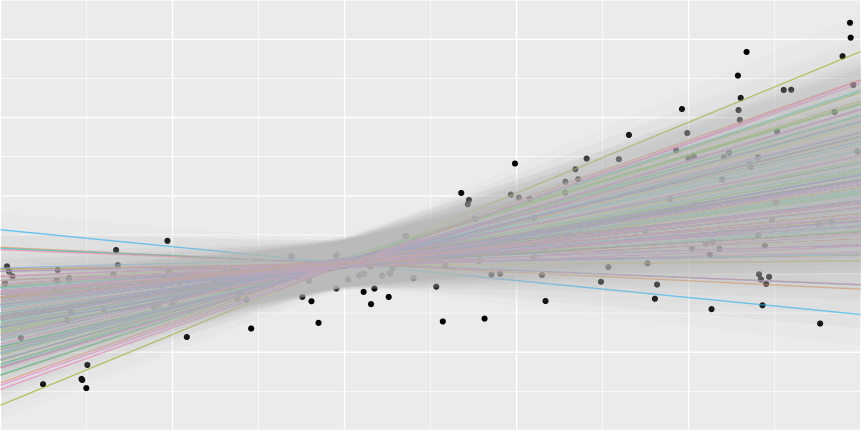
\includegraphics[width=15.65in]{uncertainty2} 

}

\caption{Posterior predictive distribution. Each line is produced by sampling from the posterior on the weights, the shading indicating the respective scales (= the learned spread in the data).}\label{fig:unnamed-chunk-2}
\end{figure}

~

~

\hypertarget{example-variational-autoencoder}{%
\subsection{Example: Variational
autoencoder}\label{example-variational-autoencoder}}

\begin{itemize}
\tightlist
\item
  Encoder and decoder both are sequential models, joined via the
  functional API
\item
  The last layer of the encoder adds a KL loss so we can simply fit with
  maximum likelihood
\end{itemize}

\small

\begin{Shaded}
\begin{Highlighting}[]
\NormalTok{encoder_model <-}\StringTok{ }\KeywordTok{keras_model_sequential}\NormalTok{() }\OperatorTok
\StringTok{  }\NormalTok{[...] }\OperatorTok
\StringTok{  }\KeywordTok{layer_multivariate_normal_tri_l}\NormalTok{(}\DataTypeTok{event_size =}\NormalTok{ encoded_size) }\OperatorTok
\StringTok{  }\KeywordTok{layer_kl_divergence_add_loss}\NormalTok{([...])}

\NormalTok{decoder_model <-}\StringTok{ }\KeywordTok{keras_model_sequential}\NormalTok{() }\OperatorTok
\StringTok{  }\NormalTok{[...] }\OperatorTok
\StringTok{ }\KeywordTok{layer_independent_bernoulli}\NormalTok{([...])}

\NormalTok{vae_model <-}\StringTok{ }\KeywordTok{keras_model}\NormalTok{(}\DataTypeTok{inputs =}\NormalTok{ encoder_model}\OperatorTok{$}\NormalTok{inputs,}
                         \DataTypeTok{outputs =} \KeywordTok{decoder_model}\NormalTok{(encoder_model}\OperatorTok{$}\NormalTok{outputs[}\DecValTok{1}\NormalTok{]))}
\NormalTok{vae_loss <-}\StringTok{ }\ControlFlowTok{function}\NormalTok{ (x, rv_x) }\OperatorTok{-}\StringTok{ }\NormalTok{(rv_x }\OperatorTok\StringTok{ }\KeywordTok{tfd_log_prob}\NormalTok{(x))}
\end{Highlighting}
\end{Shaded}

\normalsize

\hypertarget{fitting-multi-level-models-with-tfprobability}{%
\section{\texorpdfstring{Fitting multi-level models with
\texttt{tfprobability}}{Fitting multi-level models with tfprobability}}\label{fitting-multi-level-models-with-tfprobability}}

\begin{itemize}
\tightlist
\item
  Varying intercepts example from R. McElreath's ``Statistical
  rethinking''
\item
  Define model as a sequence of conditional distributions and fit with
  Hamiltonian Monte Carlo
\item
  Employs \emph{partial pooling} to make use of common features between
  tanks
\item
  See also:
  blogs.rstudio.com/tensorflow/posts/2019-05-06-tadpoles-on-tensorflow
\end{itemize}

\begin{Shaded}
\begin{Highlighting}[]
\NormalTok{model <-}\StringTok{ }\KeywordTok{tfd_joint_distribution_sequential}\NormalTok{(}
  \KeywordTok{list}\NormalTok{(}
    \KeywordTok{tfd_normal}\NormalTok{(}\DataTypeTok{loc =} \DecValTok{0}\NormalTok{, }\DataTypeTok{scale =} \FloatTok{1.5}\NormalTok{),}
    \KeywordTok{tfd_exponential}\NormalTok{(}\DataTypeTok{rate =} \DecValTok{1}\NormalTok{),}
    \ControlFlowTok{function}\NormalTok{(sigma, a_bar) }
      \KeywordTok{tfd_sample_distribution}\NormalTok{(}
        \KeywordTok{tfd_normal}\NormalTok{(}\DataTypeTok{loc =}\NormalTok{ a_bar, }\DataTypeTok{scale =}\NormalTok{ sigma),}
        \DataTypeTok{sample_shape =} \KeywordTok{list}\NormalTok{(n_tadpoles)}
\NormalTok{      ), }
    \ControlFlowTok{function}\NormalTok{(l)}
      \KeywordTok{tfd_independent}\NormalTok{(}
        \KeywordTok{tfd_binomial}\NormalTok{(}\DataTypeTok{total_count =}\NormalTok{ n_start, }\DataTypeTok{logits =}\NormalTok{ l),}
        \DataTypeTok{reinterpreted_batch_ndims =} \DecValTok{1}
\NormalTok{      )}
\NormalTok{  )}
\NormalTok{)}

\NormalTok{hmc <-}\StringTok{ }\KeywordTok{mcmc_hamiltonian_monte_carlo}\NormalTok{([...])}
\NormalTok{res <-}\StringTok{ }\NormalTok{hmc }\OperatorTok\StringTok{ }\KeywordTok{mcmc_sample_chain}\NormalTok{([...])}
\end{Highlighting}
\end{Shaded}

After fitting we see the expected shrinkage in the mean survival
estimates per tank:

\begin{figure}

{\centering 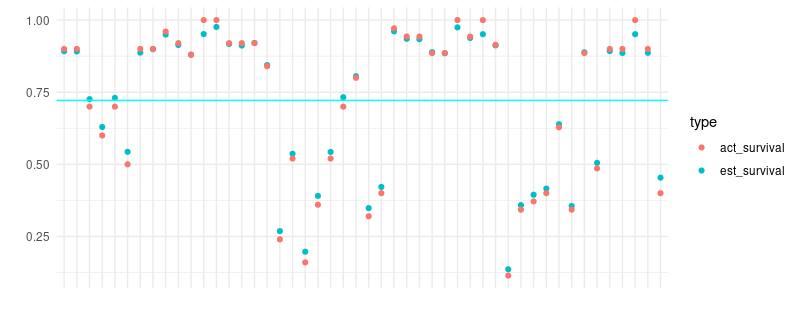
\includegraphics[width=14.55in]{shrinkage} 

}

\caption{Shrinkage in mean survival estimates due to partial pooling.}\label{fig:unnamed-chunk-4}
\end{figure}

\hypertarget{where-to-from-here}{%
\section{Where to from here?}\label{where-to-from-here}}

\begin{itemize}
\tightlist
\item
  Follow the TensorFlow for R blog: blogs.rstudio.com/tensorflow/
\item
  Documentation: rstudio.github.io/tfprobability/
\item
  Github: github.com/rstudio/tfprobability
\item
  The \emph{multiverse team} on Youtube:
  www.youtube.com/channel/UCAwJMtPx4HgmMXEDTvZBJ4A
\end{itemize}

And\ldots{} stay skeptic!

\begin{figure}

{\centering 
\includegraphics{hamster3} 

}

\caption{The skeptical hamster, popularized by Richard McElreath in his 2019 Statistical Rethinking lectures.}\label{fig:unnamed-chunk-5}
\end{figure}

``\emph{1 skeptical hamster for sale. He keeps looking at you
skeptically like you're doing it all wrong. It's driving me crazy, I
can't stand this look of reproach anymore. His name is Olaf.}''
}
\end{adjmulticols*}
%------------------ Body End ---------------------%
%end the poster
\end{document}

